\documentclass{sig-alternate}

\usepackage{tikz}
%\usetikzlibrary{plotmarks}
\usetikzlibrary{plotmarks,matrix,positioning,fit,calc}
\usepackage{amsmath}
\usepackage{graphicx}
\usepackage{xspace}
\usepackage{hyperref}
\hypersetup{
    bookmarks=false,        % show bookmarks bar?
    unicode=false,          % non-Latin characters in Acrobat’s bookmarks
    pdftoolbar=true,        % show Acrobat’s toolbar?
    pdfmenubar=true,        % show Acrobat’s menu?
    pdffitwindow=false,     % window fit to page when opened
    pdfstartview={FitH},    % fits the width of the page to the window
    pdftitle={My title},    % title
    pdfauthor={Author},     % author
    pdfsubject={Subject},   % subject of the document
    pdfcreator={Creator},   % creator of the document
    pdfproducer={Producer}, % producer of the document
    pdfkeywords={keyword1} {key2} {key3}, % list of keywords
    pdfnewwindow=true,      % links in new window
    colorlinks=true,        % false: boxed links; true: colored links
    linkcolor=black,        % color of internal links (change box color with linkbordercolor)
    citecolor=black,        % color of links to bibliography
    filecolor=black,        % color of file links
    urlcolor=black          % color of external links
}

\def \JCP{JCP\xspace}
\def \SUN{Sun Microsystems\xspace}
\def \ORACLE{Oracle\xspace}
\def \DALVIK{Dalvik\xspace}
\def \Jsr{JSR\xspace}
\def \JSR{\Jsr 292\xspace}
\def \GOOGLE{Google\xspace}
\def \ANDROID{Android\xspace}
\def \JVM{JVM\xspace}
\def \DEX{DEX\xspace}
\def \VM{VM\xspace}
\def \BSM{BSM\xspace}

\newcommand{\executeiffilenewer}[3]{%
  \ifnum\pdfstrcmp{\pdffilemoddate{#1}}{\pdffilemoddate{#2}}>0%
  {\immediate\write18{#3}}\fi%
}

\newcommand{\includesvg}[1]{%
  \executeiffilenewer{#1.svg}{#1.pdf}{inkscape -z -D --file=#1.svg --export-pdf=#1.pdf --export-latex}%
  \input{#1.pdf_tex}%
}

\newcommand{\tinyline}[3]{
  \tiny #1 &
  \tiny #2 &
  \tiny #3\\
  \hline
}

\newenvironment{listminimal}[1]%
{ \begin{minipage}{#1}%
    \medskip
    \begin{list}%
      {}%
      {%
        \setlength{\labelwidth}{0pt}%
        \setlength{\leftmargin}{0pt}%
        \setlength{\itemsep}{1pt}%
        \setlength{\parskip}{0pt}%
        \setlength{\parsep}{0pt}}%
}%
{ \\ \end{list} \end{minipage} }

\newcommand{\fixme}[1]{{\color{red} // FIXME #1}\\}

\begin{document}

\conferenceinfo{JTRES}{2014 Niagara Falls, New York USA}
%\CopyrightYear{2007} % Allows default copyright year (20XX) to be over-ridden - IF NEED BE.
%\crdata{0-12345-67-8/90/01}  % Allows default copyright data (0-89791-88-6/97/05) to be over-ridden - IF NEED BE.
% --- End of Author Metadata ---

\title{Title}
\subtitle{subtitle}

\numberofauthors{3}
\author{
  \alignauthor Gilles Roussel\\
    \affaddr{University Paris-Est Marne-la-Vallee}\\
    \email{roussel@univ-mlv.fr}
  \alignauthor Remi Forax\\
    \affaddr{University Paris-Est Marne-la-Vallee}\\
    \email{forax@univ-mlv.fr}
  \alignauthor Jerome Pilliet\\
    \affaddr{University Paris-Est Marne-la-Vallee}\\
    \email{pilliet@univ-mlv.fr}
}

\setlength{\pdfpageheight}{\paperheight}
\setlength{\pdfpagewidth}{\paperwidth}

\maketitle

\begin{abstract}
This is the text of the abstract.

bla bla bla bla bla bla bla bla bla
bla bla bla bla bla bla bla bla bla
bla bla bla bla bla bla bla bla bla
bla bla bla bla bla bla bla bla bla
bla bla bla bla bla bla bla bla bla
bla bla bla bla bla bla bla bla bla
bla bla bla bla bla bla bla bla bla

bla bla bla bla bla bla bla bla bla
bla bla bla bla bla bla bla bla bla
bla bla bla bla bla bla bla bla bla
bla bla bla bla bla bla bla bla bla
bla bla bla bla bla bla bla bla bla
bla bla bla bla bla bla bla bla bla
bla bla bla bla bla bla bla bla bla
\dots
\end{abstract}

\category{CR-number}{subcategory}{third-level}

% general terms are not compulsory anymore, 
% you may leave them out
\terms
term1, term2

\keywords
keyword1, keyword2

\section{Overview}

  \subsection{Android}

    \ANDROID is the mobile operating system created by Google.
    It's an open-source project called ``\ANDROID Open-Source Project'' (AOSP).
    In Q2 2013, \ANDROID occupies almost 80\% of the market share with more than 187 million units shipped \cite{idc-website}.
    The success of \ANDROID can be explained by an open project and an open market
    which are very attractive for devices producers, service providers and application developers \cite{ieee-butler-android-landscape}.

    \ANDROID mainly run on embedded environments like smartphones and tablets.
    Therefore, strong constraints apply to \ANDROID
    and it have to support ARM architecture and now Intel architecture.
    
    Even if hardwares supporting \ANDROID become more efficients,
    devices cannot be more powerful than desktop computer because of miniaturization.
    Being a mobile device also requires a minimal energetic consumption.
    Moreover, \ANDROID is portable system and it have to be adaptable to different devices.
    Forcing it to abstract itself from hardware.

    The \ANDROID architecture is described like a ``software stack'' (Figure \ref{ASA}).
    It's composed of:
    \begin{itemize}
      \item a modified version of the Linux kernel.
        It offers an hardware abstraction, an existing memory, process managements and a security and networking models;
      \item native libraries (C/C++)
        which provide most of features in the \ANDROID system;
      \item a virtual machine called ``\DALVIK''.
        It is a important component of \ANDROID.
        It runs applications converted to the \DEX format.
        \DALVIK uses a core API written from scratch in Java
        which can be assimilated to the version 5 or 6 of the Java API;
      \item an application framework to enable the making of \ANDROID applications;
      \item and some default applications.
    \end{itemize}

    \subsubsection{Differences between the JVM and \DALVIK}

      The main difference between these two machines is that \DALVIK is register based while the \JVM is stack based.
      A stack based virutal machine (VM) uses more instructions to manipulate data and to implement Java code than a register based VM.
      But the register based VM instructions tends to be larger in terms of code size\cite{ieee-paul-kundu-energy-perspective}.

      \begin{figure}[!h]
%         \centering 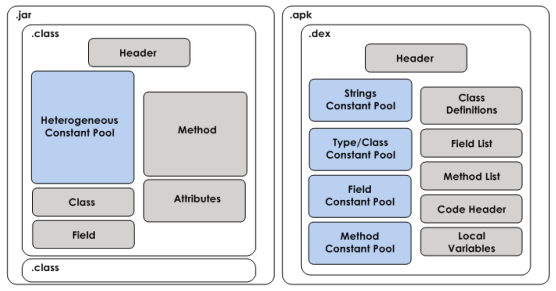
\includegraphics[width=\columnwidth]{structure-jar-apk.png}
        \centering \resizebox{1\linewidth}{!}{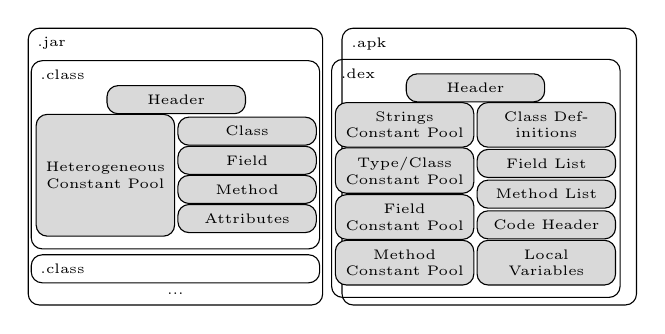
\begin{tikzpicture}[font=\tiny]
  \tikzset{every node/.style={rounded corners}}
  \node[rectangle, draw=black, align=left, text width=1.38in, inner ysep=5em] (jar) at (-.01,-.75){};
  \node[below right] at (jar.north west) {.jar};
  \node[rectangle, draw=black, align=left, text width=1.35in, inner ysep=3.4em] (class) at (-.01,-.6){};
  \node[below right] at (class.north west) {.class};
  \node[rectangle, fill=gray!30, draw=black, align=center, text width=.6in] at (0,.1){Header};
  \node[rectangle, fill=gray!30, draw=black, align=center, text width=.6in, inner ysep=1.73em] at (-.9,-.86){Heterogeneous Constant Pool};
  \node[rectangle, fill=gray!30, draw=black, align=center, text width=.6in] at (.9,-.3){Class};
  \node[rectangle, fill=gray!30, draw=black, align=center, text width=.6in] at (.9,-.67){Field};
  \node[rectangle, fill=gray!30, draw=black, align=center, text width=.6in] at (.9,-1.04){Method};
  \node[rectangle, fill=gray!30, draw=black, align=center, text width=.6in] at (.9,-1.41){Attributes};
  \node[rectangle, draw=black, align=left, text width=1.35in] at ([yshift=-.7em]class.south){.class};
  \node[below] at ([yshift=.8em]jar.south){...};
  
  \node[rectangle, draw=black, align=left, text width=1.38in, inner ysep=5em] (apk) at ([xshift=6em]jar.east){};
  \node[below right] at (apk.north west) {.apk};
  \node[rectangle, draw=black, align=left, text width=1.35in, inner ysep=4.3em] (dex) at (3.805,-.9){};
  \node[below right] at (dex.north west) {.dex};
  \node[rectangle, fill=gray!30, draw=black, align=center, text width=.6in] at (3.8,.25){Header};
  \node[rectangle, fill=gray!30, draw=black, align=center, text width=.6in] at (2.9,-.22){Strings Constant Pool};
  \node[rectangle, fill=gray!30, draw=black, align=center, text width=.6in] at (2.9,-.8){Type/Class Constant Pool};
  \node[rectangle, fill=gray!30, draw=black, align=center, text width=.6in] at (2.9,-1.39){Field\\Constant Pool};
  \node[rectangle, fill=gray!30, draw=black, align=center, text width=.6in] at (2.9,-1.97){Method Constant Pool};
  \node[rectangle, fill=gray!30, draw=black, align=center, text width=.6in] at (4.7,-.22){Class Definitions};
  \node[rectangle, fill=gray!30, draw=black, align=center, text width=.6in] at (4.7,-.71){Field List};
  \node[rectangle, fill=gray!30, draw=black, align=center, text width=.6in] at (4.7,-1.1){Method List};
  \node[rectangle, fill=gray!30, draw=black, align=center, text width=.6in] at (4.7,-1.49){Code Header};
  \node[rectangle, fill=gray!30, draw=black, align=center, text width=.6in] at (4.7,-1.97){Local Variables};
\end{tikzpicture}
}
        \caption{structure of JAR and APK files}
        \label{SJA}
      \end{figure}

      The bytecode Java is given in a ``.class'' file and contains the code of a unique class (Figure \ref{SJA}).
      The file is made of a series of tables which describes various informations, the code of the class and some other things.
      The code contains references to these tables.
      Among these tables, the constant-pool stores most of the constant values of the class (numbers or texts)
      and more evolved elements (data types, class names, attribute names, \dots).

      At the opposite, \DEX format contains all the code of the application (Figure \ref{SJA}).
      It will be loaded in one piece.
      It is a read-only format, the code cannot be changed at runtime.
      Duplicate constants such as strings used in multiple class files
      are included only once in the \DEX file to save space.
      Unlike the \JVM, \DALVIK uses one constant-pool by type of constant
      except for the primitive types which are directly encoded with the opcode.
      It leads more smaller indexes for instructions.\\

      \begin{figure}[!h]
        \centering 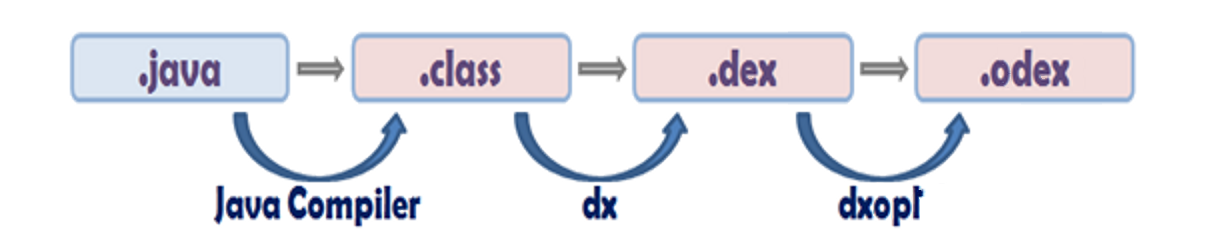
\includegraphics[width=\columnwidth]{dex-tools-chain.png}
        \caption{\ANDROID application tools-chain}
        \label{DTC}
      \end{figure}

      \DALVIK cannot directly execute Java bytecode.
      It first have to translate the Java bytecode to the \DALVIK specific one called \DEX
      which can then be optimized (\mbox{ODEX}) to save space (Figure \ref{DTC}).

    \begin{figure}[!h]
      \centering \def\svgwidth{\columnwidth} \includesvg{android-system-architecture}
      \caption{android system architecture \cite{wiki-android}}
      \label{ASA}
    \end{figure}

  \subsection{Java Specification Request 292}

    The \JSR is a request from \JCP and led by \SUN from 2006 to 2011.
    It had been integrated in 2011 in the version 7 of Java,
    modifying both the Java language specification and the \JVM specification.

    Since late 90's, a lot of language
    implementors have chosen the JVM as their target platform \cite{wiki-jvm-lang},
    for several reasons such as the size of the ecosystem,
    the presence of mature GCs and Just In Time compilers (JIT).

    The aim of this \Jsr is to ease the implementation of dynamically typed languages
    by providing a new way to do function calls that allows language implementors
    to describe a specific semantics, independantly of the semantics of the Java language.

    This \Jsr is composed of two parts, the first part, specifying the semantics of
    new opcodes and the second part defining an API: java.lang.invoke.
    This API allows to create runtime typesafe function pointers (java.lang.invoke.MethodHandle)
    and methods to combine those pointers to do things like composition, argument permutation, \dots.

    The next sections will present the new API and the new instructions but before that,
    we want to introduce an example that we will use for the rest of the paper.

    \subsubsection{Example}
      Let suppose we have the following code in Groovy \cite{lang-groovy}:

      {\scriptsize \begin{verbatim}
  def foo(a) {
    a + 2
  }

  println foo(9)
  println foo("test")
\end{verbatim} }


      It prints {\it '11'} and {\it 'test2'}.
      For the first call to {\bf foo}, {\bf a} is an integer so the symbol {\bf +} refers
      to the function {\it +(int,int)} while for the second call to {\bf foo}, {\bf a} is a string, {\bf +} refers to the function {\it +(String,String)}.

      If one try to translate this code in Java bytecode, it would be something like:

      {\scriptsize \begin{verbatim}
  def foo(a) {
    aload 0   // 0 is offset of first variable, 'a' here
    iconst_2  // load the integer constant 2
    invokevirtual Object + (I)LObject;
    areturn 
  }
\end{verbatim} }


      As you can see, the Java bytecode is typed, each instruction is prefixed 
      by the type of the operand ('a' for object, 'i' for integer, etc)
      and the method call (invokevirtual) specifies the type of the receiver and its parameters;
      an object (java/lang/Object) followed by an integer (I) ; and its return type
      which is also an object in the example.

      The code above does not work because invokevirtual is an existing Java bytecode that calls
      a virtual method using the Java semantics so the Virtual Machine or more precisely
      the bytecode verifier will check that there exists a method '+' on java.lang.Object
      that takes an integer and returns an Object. If you have already used Java, you know
      that this method does not exist. The bytecode verification will then fail.

      Another possible translation is to use a cascade of if ... instanceof.

      {\tiny \begin{verbatim}
  static Object plus(String v, Object v2) {
    return v.concat(String.valueOf(v2));
  }

  static Object plus(int v, int v2) {
    return Integer.sum(v, v2)
  }

  static Object foo(Object v, int i) {
    if (v instanceof Integer) {
      return plus((Integer)v, i);
    }
    if (v instanceof String) {
      return plus((String)v, i);
    }
    throw new Error();
  }

  public static void main(String[] args) {
    System.out.println(foo(9));
    System.out.println(foo("bar"));
  }
\end{verbatim} }


      While this code works, it supposes that all the potentials variations of + are known at compile time,
      something which is not true in most dynamic languages (Ruby, Groovy, Dart by example).
      This code can also be slow because in real languages, the number of if ... instanceof branches
      can be greater than a dozen. 

      To solve these issues, the \Jsr introduces a new bytecode named invokedynamic with no predefined
      linking semantics. It introduces also a mechanism that allows to specify the linking semantics in Java
      or any languages that can be compiled to bytecodes.
      Invokedynamic is a function call so it can simulate every other existing Java calls.
      It delegates its linking semantics to an external Java method, the bootstrap method.
      This method returns a CallSite object which is a box that contains a function pointer (MethodHandle).

      The \JSR has created a new package named\\ ``java.lang.invoke''.
      It is composed of classes MethodType, MethodHandle and CallSite.
      These classes are directly understood by the \JVM.
      All classes answer to one or more problems coming from dynamic languages optimizations or implementations.

    \subsubsection{invoke-dynamic and MethodHandle}

      The bootstrap method is called the first time the invokedynamic opcode is encountered by the interpreter,
      with the context where the opcode is located i.e.~the declaring class (encapsulated in a Lookup object),
      a symbolic name and the declared parameter types as a MethodType.
      Any subsequent execution of the invokedynamic opcode will call the function pointer
      stored inside the callsite object returned by the bootstrap method.
      
      For our example, the code of {\bf foo} with invokedynamic is

      {\tiny \begin{verbatim}
  def foo(a) {
    aload 0
    iconst_2 
    invokedynamic  + (LObject;I)LObject;
      bsm: invokestatic RT.bootstrap:(LMethodHandles$Lookup;LString;LMethodType;)LCallSite;
    areturn 
  }
\end{verbatim} }

      The first time that {\bf foo} is executed, the bootstrap method of the class RT will be called, with a lookup corresponding to the class containing {\bf foo},
      the string {\bf ``+''} and a MethodType corresponding to the descriptor ``(LObject;I)LObject;'' (Figure \ref{fooBSM}).

      \begin{figure}[!h]
        \centering {\scriptsize \begin{verbatim}
import static java.lang.invoke.MethodType.*

public class RT {
    ...
  private static final Lookup lookup = MethodHandles.lookup();

  public static CallSite bootstrap(
      Lookup caller, String name, MethodType type)
      throws IllegalAccessException, NoSuchMethodException {
    MethodType mt = methodType(Object.class,
                               MutableCallSite.class,
                               Object[].class);
    MethodHandle mh =
      lookup.findStatic(BootStraps.class, "change", mt);
    return new CSMutableBind(type, mh);
  }
    ...
}
\end{verbatim} }

        \caption{Example - bootstrap method.}
        \label{fooBSM}
      \end{figure}

      Moreover, invokedynamic comes with an API that allows to create several data patterns
      dynamically and lazily like for example a tree of if ... instanceof branches.

    \subsubsection{MethodType}

      A method type represents the types of the arguments and the return value accepted and returned by a method handle,
      or expected by a method handle caller.
      This class represents a method signature.

      \begin{figure}[!h]
        \centering {\scriptsize \begin{verbatim}
import static java.lang.invoke.MetodType.*;

public class RT {
    ...
  private static Object plus(int a, int b) {
    return a + b;
  }

  private static Object plus(String a, int b) {
    return a + b;
  }

  private static boolean check(Object value, Class<?> clazz) {
    return value.getClass() == clazz;
  }

  private static final MethodHandle TARGET_INT;
  private static final MethodHandle TARGET_STRING;
  private static final MethodHandle TARGET_CHECK;

  static {
    try {
      MethodType mti =
        methodType(Object.class, int.class, int.class);
      TARGET_INT =
        lookup.findStatic(BootStraps.class, "plus", mti);

      MethodType mts =
        methodType(Object.class, String.class, int.class);
      TARGET_STRING =
        lookup.findStatic(BootStraps.class, "plus", mts);

      MethodType mtc =
        methodType(boolean.class, Object.class, Class.class);
      TARGET_CHECK =
        lookup.findStatic(BootStraps.class, "check", mtc);
    } catch (NoSuchMethodException|IllegalAccessException e) {
      throw new AssertionError(e);
    }
    ...
}
\end{verbatim} }

        \caption{Example - methods with method types.}
        \label{fooMTS}
      \end{figure}

      All method types are immutable and interned.
      It can only be created by factory methods.
      In our example, we need three method types (Figure \ref{fooMTS}), one for each method that we have to call:
      the ``check'' method; and the two methods ``plus''.

    \subsubsection{MethodHandle / MethodHandles}
      \label{MH}

      A method handle is a runtime type checked, directly executable reference to
      either an underlying method, constructor, field, or similar low-level operation.
      It also represents a combiner operation that takes one or more method handles as input and
      applies an operation like an argument transformation, a function compositions, etc.
      The former kind of method handle is called {\it direct method handle},
      the later is called a {\it combiner method handle}.

      To guarantee runtime type safety, each method handle embodies a method type (of type MethodType)
      that describes the parameter types and the return type that a method handle accepts.
      When a method handle is called, the method type is checked using different semantics depending on the
      type of call.

      There are two kinds of method handle call semantics:
      \begin{itemize}
        \item the exact call semantics, in that case, the declared type of the arguments (and return value) at a call site
              must be exactly the same as the types of the method type.
        \item the generic call semantics, in that case, the arguments can be converted using widening primitive conversions,
              boxing and unboxing conversions and varargs conversions as defined in the Java Language Specification.
      \end{itemize}
      None of these semantics implements the calling semantics as defined by the Java Virtual Machine Specification
      for classical Java method calls like invokestatic or invokevirtual
      \footnote{There is also a minor difference between the generic call semantics and the call semantics of
        the Java Language Specification if the method is a varargs and the call as the same number of parameters as the method.
        The generic call semantics will not try to do the varargs conversion if the last parameter is not an array.},
      the exact call semantics is more strict, and the generic call semantics is more permissive.

      We can distinguish two kinds of method handle:
      the one which do a direct call to a method or to a field access, this method handle is direct;
      and the one which manipulates arguments called ``combiners''.
      The combiners contain at least one direct method handle and can be represented by a tree.

      In our example, we want to call a method which takes an Object and an integer and returns an Object.
      We need to resolve the right method to call (addition or concatenation).
      In order to do that, we write a method which will create the right method handle called {\bf change} (detailed after).

      \begin{figure}[!h]
        \centering {\tiny \begin{verbatim}
public class RT {
    ...
  private static class CSMutableBind extends MutableCallSite {
    CSMutableBind(MethodType type, MethodHandle mh) {
      super(type);
      setTarget(mh.bindTo(this)
                  .asCollector(Object[].class, type.parameterCount())
                  .asType(type));
    }
  }
    ...
}
\end{verbatim} }
        \caption{Example - mutable call site.}
        \label{fooMCS}
      \end{figure}

      We need to adapt the arguments to move from an Object and an integer to a CallSite and an array of Object.
      To do this we convert arguments (asType), we collect them to form the array of Objects (asCollector) and we add the call site at first argument (bindTo) (Figure \ref{fooMCS}).

      \noindent This adaptation forms the tree of the Figure \ref{ast1}.

      % graph 1
      \begin{figure}[!h]
        \centering \resizebox{.7\linewidth}{!}{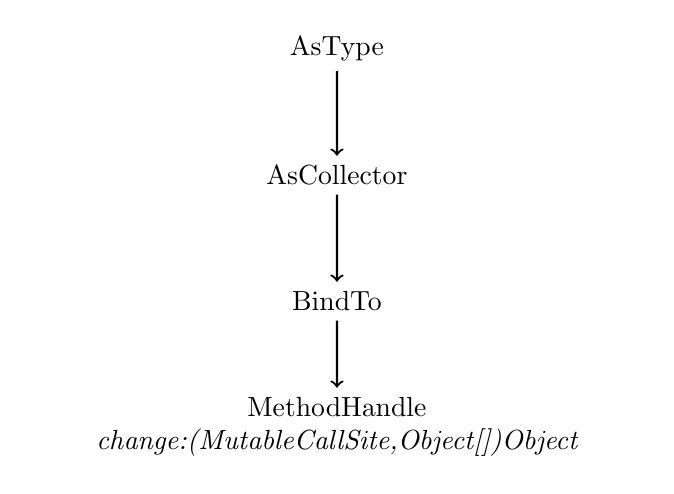
\begin{tikzpicture}[scale=1.6]
  \node[text width=3in,align=center](A1) at (2,-2){AsType};
  \node[text width=3in,align=center](A2) at (2,-3){AsCollector};
  \node[text width=3in,align=center](A3) at (2,-4){BindTo};
  \node[text width=3in,align=center](A4) at (2,-5){MethodHandle\\{\it change:(MutableCallSite,Object[])Object}};

  \draw[thick,->](A1) -- (A2);
  \draw[thick,->](A2) -- (A3);
  \draw[thick,->](A3) -- (A4);
\end{tikzpicture}
}
        \caption{Method handles tree - bootstrap method.}
        \label{ast1}
      \end{figure}

      When the call site is created, the method handle tree is called, so the {\bf change} method (Figure \ref{fooCHANGE}) is called.
      This method takes a look at the dynamic type of {\bf a} (let say an integer),
      finds the corresponding implementation of the {\bf plus} method
      and then re-links a method handles tree represented by a combiner called {\bf GuardWithTest}.
      This combiner uses the {\bf check} method to verify the class of {\bf a}.
      If the type of {\bf a} is an integer it will directly call the same implementation of {\bf plus};
      otherwise it uses the previous method handle tree.

      \begin{figure}[!h]
        \centering {\scriptsize \begin{verbatim}
  private static Object change(
      MutableCallSite callSite, Object[] arguments)
      throws Throwable {
    MethodHandle target;
    MethodType type = callSite.type();
    Class<?> aClass = arguments[0].getClass();
    if (aClass == Integer.class) {
      target = TARGET_INT.asType(type);
    } else if (aClass == String.class) {
      target = TARGET_STRING.asType(type);
    } else {
      throw new LinkageError("bad receiver class");
    }
    MethodHandle test = MethodHandles
        .insertArguments(TARGET_CHECK, 1, aClass);
    test = MethodHandles
        .dropArguments(test, 1, type.parameterType(1));
    callSite.setTarget(MethodHandles
        .guardWithTest(test, target, callSite.getTarget()));
    return target.invokeWithArguments(arguments);
  }
\end{verbatim} }

        \caption{Example - ``change'' method.}
        \label{fooCHANGE}
      \end{figure}

      To call the {\bf check} method, we have to adapt arguments.
      The stack contains an Object and an integer, we need an Object and a java.lang.Class.
      So we have to drop the integer (dropArguments) and insert the class (insertArguments).
      This adaptation forms the tree of the Figure \ref{ast2}.

      % graph 2
      \begin{figure}[!h]
        \hspace{-.6in} \resizebox{1.3\linewidth}{!}{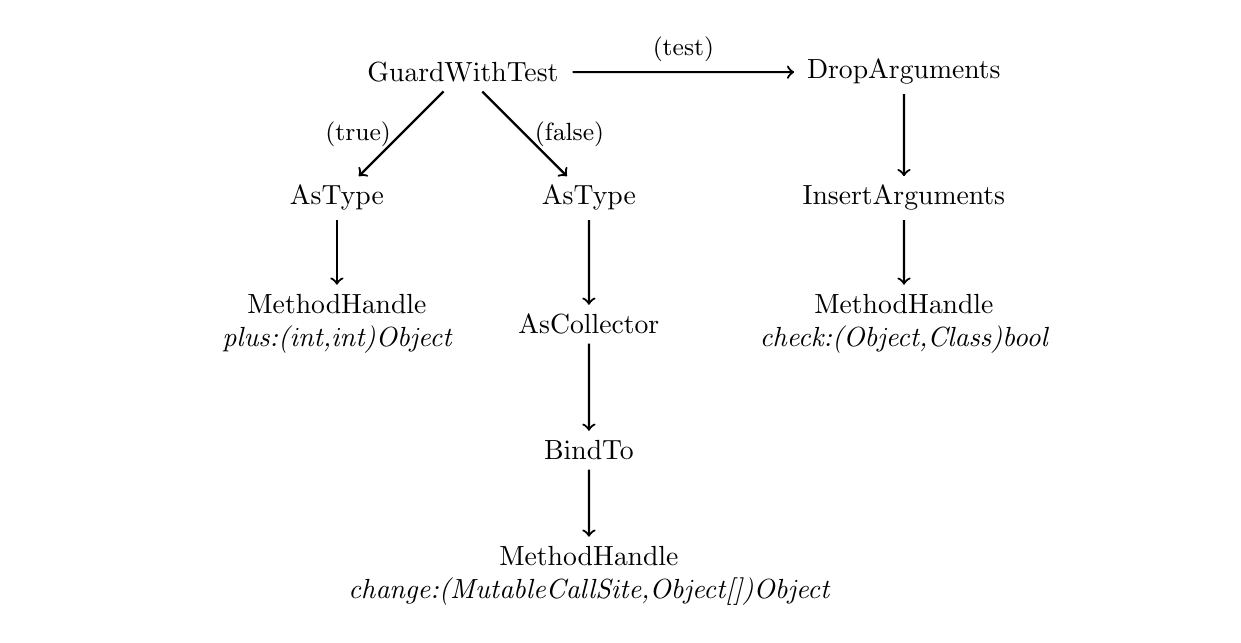
\begin{tikzpicture}[scale=1.6]
  \node[text width=3in,align=center](A1) at (2,-2){AsType};
  \node[text width=3in,align=center](A2) at (2,-3){AsCollector};
  \node[text width=3in,align=center](A3) at (2,-4){BindTo};
  \node[text width=3in,align=center](A4) at (2,-5){MethodHandle\\{\it change:(MutableCallSite,Object[])Object}};

  \node[text width=1in,align=center](G1) at (1,-1){GuardWithTest};

  \node[text width=3in,align=center](B1) at (0,-2){AsType};
  \node[text width=3in,align=center](B2) at (0,-3){MethodHandle\\{\it plus:(int,int)Object}};

  \node[text width=1in,align=center](C1) at (4.5,-1){DropArguments};
  \node[text width=3in,align=center](C2) at (4.5,-2){InsertArguments};
  \node[text width=3in,align=center](C3) at (4.5,-3){MethodHandle\\{\it check:(Object,Class)bool}};

  \draw[thick,->](A1) -- (A2);
  \draw[thick,->](A2) -- (A3);
  \draw[thick,->](A3) -- (A4);
  \draw[thick,->](B1) -- (B2);

  \draw[thick,->](C1) -- (C2);
  \draw[thick,->](C2) -- (C3);
  \draw[thick,->](G1) -- node[right] {\small (false)} (A1);
  \draw[thick,->](G1) -- node[left]  {\small (true)}  (B1);
  \draw[thick,->](G1) -- node[above] {\small (test)}  (C1);
\end{tikzpicture}
}
        \caption{Method handles tree - first call (integer).}
        \label{ast2}
      \end{figure}

      If 'a' is a string, the method {\bf change} is called again,
      installing a new method handle tree testing if 'a' is a string in order to call {\it plus(String,int)Object}.
      This adaptation form the tree of the Figure \ref{ast3}.

      % graph 3
      \begin{figure*}
        \centering \resizebox{.9\linewidth}{!}{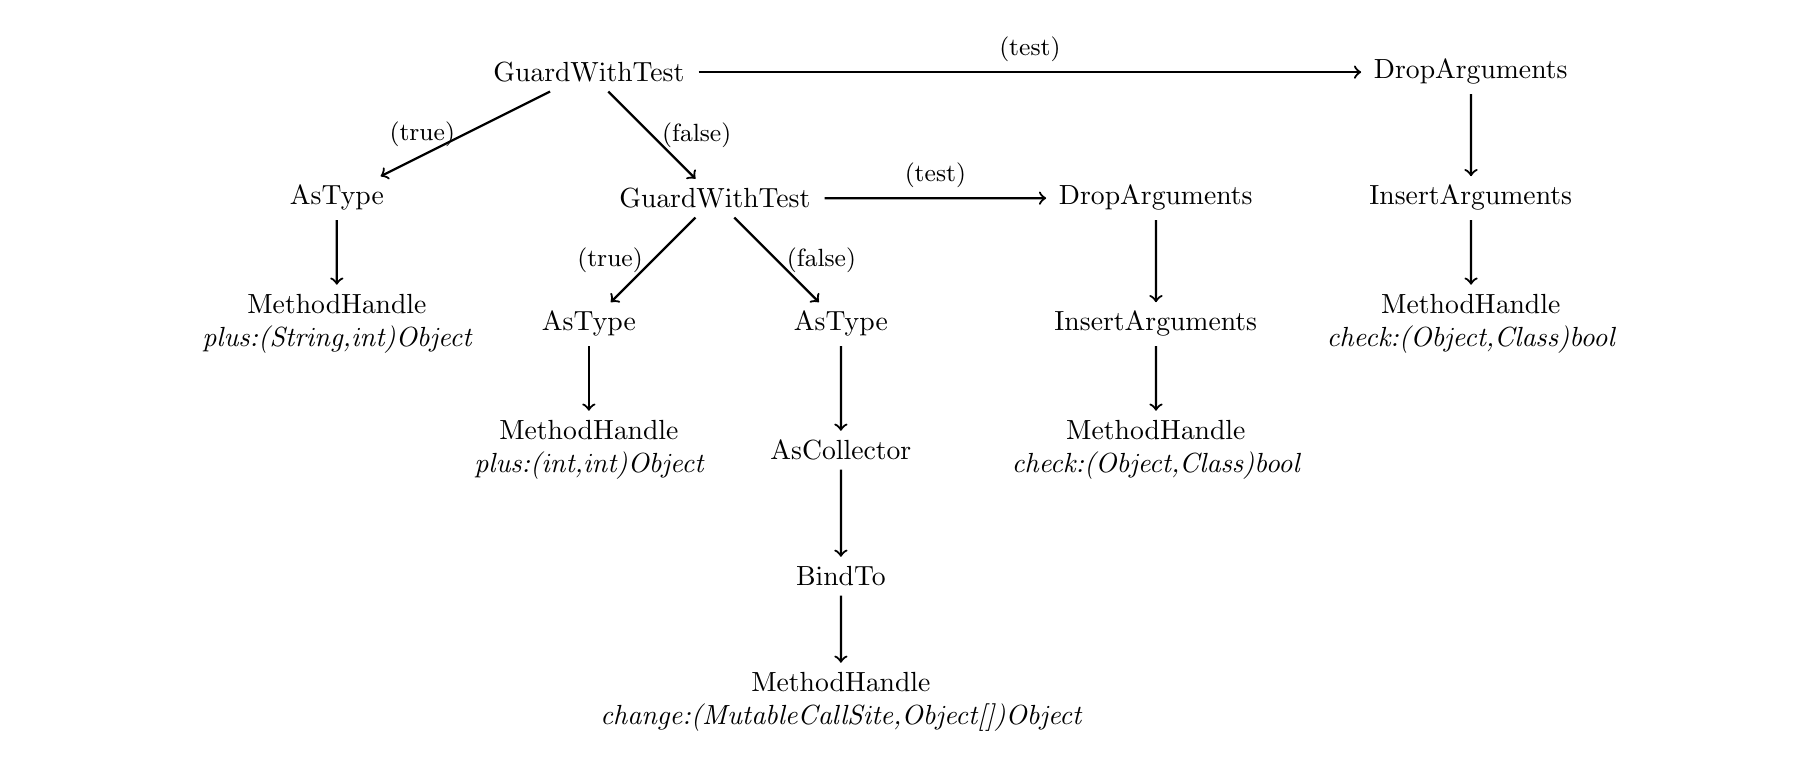
\begin{tikzpicture}[scale=1.6]
    \node[text width=3in,align=center](A1) at (2,-2){AsType};
    \node[text width=3in,align=center](A2) at (2,-3){AsCollector};
    \node[text width=3in,align=center](A3) at (2,-4){BindTo};
    \node[text width=3in,align=center](A4) at (2,-5){MethodHandle\\{\it change:(MutableCallSite,Object[])Object}};

    \node[text width=1in,align=center](G1) at (1,-1){GuardWithTest};

    \node[text width=3in,align=center](B1) at (0,-2){AsType};
    \node[text width=3in,align=center](B2) at (0,-3){MethodHandle\\{\it plus:(int,int)Object}};

    \node[text width=1in,align=center](C1) at (4.5,-1){DropArguments};
    \node[text width=3in,align=center](C2) at (4.5,-2){InsertArguments};
    \node[text width=3in,align=center](C3) at (4.5,-3){MethodHandle\\{\it check:(Object,Class)bool}};

    \node[text width=1in,align=center](G2) at (0, 0){GuardWithTest};

    \node[text width=3in,align=center](D1) at (-2,-1){AsType};
    \node[text width=3in,align=center](D2) at (-2,-2){MethodHandle\\{\it plus:(String,int)Object}};

    \node[text width=1in,align=center](E1) at (7, 0){DropArguments};
    \node[text width=3in,align=center](E2) at (7,-1){InsertArguments};
    \node[text width=3in,align=center](E3) at (7,-2){MethodHandle\\{\it check:(Object,Class)bool}};

    \draw[thick,->](A1) -- (A2);
    \draw[thick,->](A2) -- (A3);
    \draw[thick,->](A3) -- (A4);
    \draw[thick,->](B1) -- (B2);

    \draw[thick,->](C1) -- (C2);
    \draw[thick,->](C2) -- (C3);
    \draw[thick,->](G1) -- node[right] {\small (false)} (A1);
    \draw[thick,->](G1) -- node[left]  {\small (true)}  (B1);
    \draw[thick,->](G1) -- node[above] {\small (test)}  (C1);

    \draw[thick,->](D1) -- (D2);
    \draw[thick,->](E1) -- (E2);
    \draw[thick,->](E2) -- (E3);
    \draw[thick,->](G2) -- node[right] {\small (false)} (G1);
    \draw[thick,->](G2) -- node[left]  {\small (true)}  (D1);
    \draw[thick,->](G2) -- node[above] {\small (test)}  (E1);
\end{tikzpicture}
}
        \caption{Method handles tree - second call (string).}
        \label{ast3}
      \end{figure*}

    \subsubsection{CallSite}

      A CallSite is a holder for a variable MethodHandle, which is called its target.
      An invokedynamic instruction linked to a CallSite delegates all calls to the site's current target.
      A CallSite may be associated with several invokedynamic instructions,
      or it may be ``free floating'', associated with none.\\

      It has three immediate, concrete subclasses that may be either instantiated or subclassed:
      \begin{enumerate}
        \item \textbf{ConstantCallSite} : If a mutable target is not required.
        \item \textbf{MutableCallSite}  : If a mutable target is required.
        \item \textbf{VolatileCallSite} : If a mutable target is required which has volatile variable semantics.
      \end{enumerate}
      A non-constant call site may be relinked by changing its target, calling ``setTarget'' on the CallSite.
      The new target must have the same type as the previous one.

\section{Android 292}
  Currently only the desktop and the server version (HotSpot, J9, \dots) of the JVM have a complete implementation of the JSR 292.
  These implementations use mechanisms that we cannot reuse with \DALVIK (code generation, rewriting, \dots)
  because of the power costs and computing restrictions.
  For this reason, \DALVIK is seen like a specific virtual machine from language developers.
    
  Our solution is to make an implementation of the JSR 292 for Android but,
  because Android have many constraints from its environment,
  we have to reinterpret the JSR.
  The API stays the same, but the VM specification does not.

  The next sections talk about how we made this solution.
  We will explain our new DEX format with a new header, classes modification
  \dots~and how we maintain compatibility with post-invokedynamic APKs (cf.~\ref{newDEX}).
  How we represent the new constants and new instructions (cf.~\ref{newConst}).
  And we will detail most important implementation parts: method handles, invoke instructions, \dots~(cf.~\ref{implD}).
  At the end, we will descibe our results in terms of execution time and code size.\\

  Our solution is not necessary fast, we have focussed on the conformance of the \JSR.
  And to simplify the implementation, we have just integrated our solution in the ``portable'' interpreter written in C and not in assembly code.
  
\section{A new DEX format}
\label{newDEX}

  New instructions and new constants imply a new format of DEX file.
  Each DEX file version have a version number, our one is number 292.
  We enhance the opcode set, add constant-pools and change the header of classes.
  But we have to maintain the compatibility with the DEX files created before our version.

  \subsection{opcodes / constants}
    The \JSR needs two new constants (``const-methodtype'' and ``const-methodhandle'') and a new instruction (``invoke-dynamic'').
    Regarding the two methods ``invoke'' and ``invokeExact'', we made the choice to add two new instructions:
    ``invoke-exact'' for the ``invokeExact'' method and ``invoke-generic'' for the ``invoke'' method.
    It is the program ``dx'' (Figure \ref{DTC}) which transforms virtual calls to ``invokeExact'' and ``invoke'' to instructions.

  \subsection{constant-pools}
    \label{CP}

    \DALVIK have a constant pool for each entry type.
    We have to add constant pool for each entry we need:
    MethodType, MethodHandle, InvokeDynamic and Bootstrap Arguments (Figure \ref{SNA}).

    \begin{figure}[!h]
%       \centering 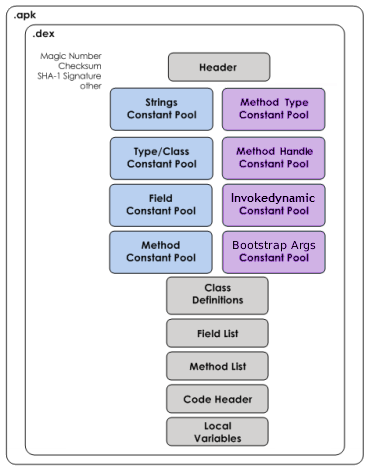
\includegraphics[width=.5\columnwidth]{structure-apk-292.png}
      \centering \resizebox{.55\linewidth}{!}{\begin{tikzpicture}[font=\tiny]
  \tikzset{every node/.style={rounded corners}}
  \node[rectangle, draw=black, align=left, text width=1.38in, inner ysep=8.6em] (apk) at ([xshift=6em]jar.east){};
  \node[below right] at (apk.north west) {.apk};
  \node[rectangle, draw=black, align=left, text width=1.35in, inner ysep=8em] (dex) at (3.805,-.9){};
  \node[below right] at (dex.north west) {.dex};
  \node[rectangle, fill=gray!30, draw=black, align=center, text width=.6in] at (3.8,1.3){Header};
  \node[rectangle, fill=gray!30, draw=black, align=center, text width=.6in] at (2.9,.83){Strings Constant Pool};
  \node[rectangle, fill=gray!30, draw=black, align=center, text width=.6in] at (2.9,.25){Type/Class Constant Pool};
  \node[rectangle, fill=gray!30, draw=black, align=center, text width=.6in] at (2.9,-.34){Field\\Constant Pool};
  \node[rectangle, fill=gray!30, draw=black, align=center, text width=.6in] at (2.9,-.92){Method Constant Pool};
  \node[rectangle, fill=green!30, draw=black, align=center, text width=.6in] at (4.7,.83){MethodType Constant Pool};
  \node[rectangle, fill=green!30, draw=black, align=center, text width=.6in] at (4.7,.25){MethodHandle Constant Pool};
  \node[rectangle, fill=green!30, draw=black, align=center, text width=.6in] at (4.7,-.34){Invokedynamic Constant Pool};
  \node[rectangle, fill=green!30, draw=black, align=center, text width=.6in] at (4.7,-.92){BootstrapArgs Constant Pool};
  \node[rectangle, fill=gray!30, draw=black, align=center, text width=.6in] at (3.8,-1.50){Class Definitions};
  \node[rectangle, fill=gray!30, draw=black, align=center, text width=.6in] at (3.8,-1.97){Field List};
  \node[rectangle, fill=gray!30, draw=black, align=center, text width=.6in] at (3.8,-2.33){Method List};
  \node[rectangle, fill=gray!30, draw=black, align=center, text width=.6in] at (3.8,-2.69){Code Header};
  \node[rectangle, fill=gray!30, draw=black, align=center, text width=.6in] at (3.8,-3.16){Local Variables};
\end{tikzpicture}
}
      \caption{structure of new APK files}
      \label{SNA}
    \end{figure}

    The MethodType entry contains an index into the prototype constant pool.
    The MethodHandle entry contains the method handle kind (cf.~\ref{MH})
    and an index into the method or the field constant pool, according to the kind.
    The InvokeDynamic entry contains indexes into the strings, the prototype,
    the method handle and the bootstrap arguments constant pools.
    And the Bootstrap arguments entry contains its arguments number
    and a data block representing the arguments.
    Each argument is encoded with a tag
    followed by a constant pool index or the primitive value according to the tag (Figure \ref{CPentries}).

    \begin{figure}[!h]
      \centering {\tiny \begin{verbatim}
  /*
   * Direct-mapped "methodType_id_item".
   */
  struct DexMethodTypeId {
    u2  protoIdx;           /* index into protoIds */
  };
\end{verbatim} }
      \centering {\scriptsize \begin{verbatim}
  /*
   * Direct-mapped "methodHandle_id_item".
   */
  struct DexMethodHandleId {
    u4  kind;
    u4  memberIdx;    /* index into methodIds or fieldIds */
  };
\end{verbatim} }

      \centering {\scriptsize \begin{verbatim}
  /*
   * Direct-mapped "indy_id_item".
   */
  struct DexInvokeDynamicId {
    u4 nameIdx;       /* index into stringIdx */
    u2 typeIdx;       /* index into protoIdx */
    u2 methodHandleIdx;
    u4 bsmargOff;
  };
\end{verbatim} }

      \centering {\scriptsize \begin{verbatim}
  /* Direct-mapped "bsmArgsList_id_item". */
  struct DexBsmArgsListId {
    u4 size;          /* number of argument couples */
    u1 arguments[1];  /* array of couple {type,[idx|value]} */
  };
\end{verbatim} }

      \caption{Constant pool entries.}
      \label{CPentries}
    \end{figure}

  \subsection{Class header}

    A call site is bound to an instruction so it's not interresting to store them into a constant-pool.
    So we have to create a table that contains the call sites.
    We have three ways to store the call sites: in the DEX header; in the method which contains the instruction or in the class where the method is.
    As a reminder, a DEX file describes all the classes of a program, and a class can have at most 65535 methods (cf.~jvms 4.11).
    A method can contains a lot of instructions and the table of call sites can quickly overflow.
    The best solution is to store the call sites in the method, but \DALVIK does not have a lazy mecanism to create methods.
    All methods are created when the class was created.
    Eventually, we store the table in the header of each class.

  \subsection{retro-compatibility}
    Our \ANDROID version understands post-invokedynamic APK.
    We need to modify the APK to add missing constant pools and CallSite tables.
    However an APK is read-only.
    But the installation time does optimizations and has to modify the APK using ``dexopt'' (Figure \ref{DTC}).
    We take advantage to the installation time to add our work.
    We just simulate an APK without MethodHandle, MethodType, CallSite, \dots~%
    Only the DEX header and classes header change, we add empty constant pools to the header
    and an empty table in each class representing the CallSite table.
    No offset changes, just the size of the DEX header and classes.

\section{New opcodes}
\label{newConst}
  \subsection{New constants}

    We can create constant method handles only with the ``const-methodhandle'' instruction (Figure \ref{MTMHldc}) or in the arguments of a bootstrap method.
    The method handle instructions are rarely used and a bootstrap method is called once.
    Therefore it's not necessary to have a cache for method handles resolved.
    Resolve a method handle consists to find its informations into the constant-pool and create it.
    This creation can only do in Java, an up call is necessary.

    Comparing method types is common on the VM.
    To simplify and optimize these tests, we need to maintain a cache which make sure that two method types with the same signature are identicals.
    A method type can be create in Java or by the VM so the cache run in Java and only Java can create a method type (the VM does an up call).
    All method types are store in the cache and a test between two method types becomes a simply equality test.
    Resolve a method type consists to find its prototype in the constant-pool and call Java to find it or create it.
    We distinguish two types of method type: some are used by the VM (strong) and must not be freed by the GC; the others (weak) can be freed by the GC if necessary.

    \begin{figure}[!h]
      \centering \begin{tabular}{|l|l|l|}
  \hline
  \tinyline
    {3e}{21c}
    {%
      \begin{listminimal}{6cm}
        \item const-methodtype vA, methodtype$@$BBBB
          \item \hspace{.2in}A : destination register or pair (4 bits)
          \item \hspace{.2in}B : methodtype reference index (16 bits)
      \end{listminimal}
    }
  \tinyline
    {3f}{21c}
    {%
      \begin{listminimal}{6cm}
        \item const-methodhandle vA, methodhandle$@$BBBB
          \item \hspace{.2in}A : destination register or pair (4 bits)
          \item \hspace{.2in}B : methodhandle reference index (16 bits)
      \end{listminimal}
    }
\end{tabular}

      \caption{methodtype and methodhandle constant}
      \label{MTMHldc}
    \end{figure}

  \subsection{New invoke instructions}
    Each instruction have two representations: a ``normal'' form and a ``range'' form.
    The ``normal'' form represents the instruction with at most 5 registers.
    And the ``range'' form can have at most 65535 registers.
    Each register is considered 32 bits wide.

    \subsubsection{invoke-exact and invoke-generic}

      invoke-exact and invoke-generic (Figure \ref{INGEins}) contain an index in the constant-pool of method types.
      This method type represents the order and types of the arguments passed to the instruction, the first argument excluded.
      The first argument is the method handle we have to call.\\

      \begin{figure}[!h]
        \centering \begin{tabular}{|c|c|c|}
  \hline
  \tinyline{opcode}{format}{description}
  \tinyline
    {40..41}{35c}
    {
      \begin{listminimal}{6cm}
        \item invoke-\textit{kind} \{vC, vD, vE, vF, vG\},
        \item \hspace{.6in} methodtype$@$BBBB
          \item \hspace{.1in}40 : invoke-exact
          \item \hspace{.1in}41 : invoke-generic
            \item \hspace{.2in}A : argument word count (4 bits)
            \item \hspace{.2in}B : methodtype reference index (16 bits)
            \item \hspace{.2in}C..G : argument registers (4 bits each)
      \end{listminimal}
    }
  \tinyline
    {42..43}{3rc}
    {
      \begin{listminimal}{6cm}
        \item invoke-\textit{kind}/range \{vCCCC .. vNNNN\},
        \item \hspace{.6in} methodtype$@$BBBB
          \item \hspace{.1in}42 : invoke-exact/range
          \item \hspace{.1in}43 : invoke-generic/range
            \item \hspace{.2in}A : argument word count (8 bits)
            \item \hspace{.2in}B : methodtype reference index (16 bits)
            \item \hspace{.2in}C : first argument register (16 bits)
            \item \hspace{.2in}N = A + C - 1
      \end{listminimal}
    }
\end{tabular}

        \caption{invoke-generic/exact instruction}
        \label{INGEins}
      \end{figure}

    \subsubsection{invoke-dynamic}

      An invoke-dynamic (Figure \ref{INDYins}) contains an integer corresponding to the call site number and an index in the constant-pool of invoke-dynamic.
      This entry in the invoke-dynamic constant pool have all informations we need to treat this instruction: bootstrap method, arguments, \dots (cf.~\ref{CP}).
      A new opcode format has been added.

      \begin{figure}[!h]
        \centering \begin{tabular}{|l|l|l|l|}
  \hline
  \tinyline
    {73}{55ci}
    {
      \begin{listminimal}{6cm}
        \item 73 : invoke-dynamic \{vC, vD, vE, vF, vG\}, indy$@$BBBB, \#ZZZZZZZZ
          \item \hspace{.2in}A:C-G : like invoke-exact and invoke-generic
          \item \hspace{.2in}B : invoke-dynamic reference index (16 bits)
          \item \hspace{.2in}Z : callsite\_index (32 bits)
      \end{listminimal}
    }
  \tinyline
    {79}{5rci}
    {
      \begin{listminimal}{6cm}
        \item 79 : invoke-dynamic/range \{vCCCC .. vNNNN\}, indy$@$BBBB, \#ZZZZZZZZ
          \item \hspace{.2in}A:C-N : like invoke-exact/range and invoke-generic/range
          \item \hspace{.2in}B : invoke-dynamic reference index (16 bits)
          \item \hspace{.2in}Z : callsite\_index (32 bits)
      \end{listminimal}
    }
\end{tabular}

        \caption{invoke-dynamic instruction}
        \label{INDYins}
      \end{figure}

\section{Implementation details}
\label{implD}

    \subsection{MethodHandle}
      Method handles can be divide in three parts (Figure \ref{mhHier}):
      direct method handles which are treated by a call to the method {\bf invoke} or {\bf invokeExact};
      combiners which require specific treatments;
      and invokers which simulate an ``invoke'' or ``invokeExact'' call.

      \begin{figure}[!h]
        \centering \resizebox{.7\linewidth}{!}{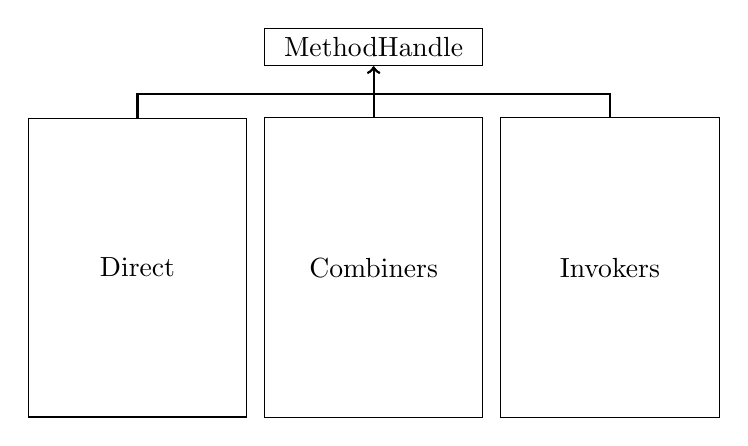
\begin{tikzpicture}[scale=2]
  \node[rectangle, draw=black, align=center, text width=1in](A1) at (0,0){MethodHandle};
  \node[rectangle, draw=black, align=center, text width=1in, inner ysep=.7in](A2) at (-1.5,-1.4){Direct};
  \node[rectangle, draw=black, align=center, text width=1in, inner ysep=.7in](A3) at (   0,-1.4){Combiners};
  \node[rectangle, draw=black, align=center, text width=1in, inner ysep=.7in](A4) at ( 1.5,-1.4){Invokers};

  \draw[thick,<-](A1) -- ++(0,-0.3) -| (A2);
  \draw[thick,<-](A1) -- ++(0,-0.3) -| (A3);
  \draw[thick,<-](A1) -- ++(0,-0.3) -| (A4);
\end{tikzpicture}
}
        \caption{Method handles hierarchy.}
        \label{mhHier}
      \end{figure}

      Each part gathers together different kinds of method handle.
      The ``direct'' part contains all method handles which do an invoke (virtual, direct, static, \dots)
      and a field access (get, put) with a possible ``static'' and ``volatile'' form.
      The ``combiner'' part
      We need to differentiate all kinds of direct method

      And we made a specific interpreter, written in Java, which executes method handle trees (combiners).

    \subsection{invoke instructions}
      All new instructions work with a method handle so we made a method, inside the interpreter, which treats a method handle.
      It invokes the method, gets or sets a field and calls the method handle interpreter depending to the kind of the method handle.
      It also uses the interpreter mecanism to store the return value.
      This method is called ``invokeMethodHandle''.

    \subsubsection{invoke-exact and invoke-generic}
      invoke-exact is the instruction with the most simple implementation.
      If the two method types (contained in the instruction and in the method handle) are equals, we call the method handle.
      Else an exception is thrown.\\
      
      invoke-generic works like an invoke-exact but if the method types differ, we try to adapt arguments.
      Differents treatment can be done:
      if the number of arguments is the same between the two method types, we try to convert arguments;
      else if we have a variadic signature, we collect and convert arguments to match the method type of the method handle.
      else an exception is thrown.
      When the arguments match the method signature, we call the method handle.
  
    \subsubsection{invoke-dynamic}
      The call site is found in the current class but if it's the first time we read this instruction, the call site is not created.
      So we need to call the bootstrap method associated to the instruction first.
      So we decode the arguments of the bootstrap method and do an up call to a method called ``callBootstrapMethod'' (Figure \ref{implBSM}).
      It returns a call site that we store in the class.

      A bootstrap method needs at least three arguments:
      a lookup (Lookup), that it's a security token object encapsulating access rigths of class containing the invoke-dynamic opcode;
      an arbitrary name (String) specified as parameter of the invokedynamic opcode;
      a method type (MethodType), that it's a reified object of the descriptor specified as parameter of the invoke-dynamic opcode;
      and any constant values specified as bootstrap arguments of the invoke-dynamic opcode.

      \begin{figure}[!h]
        \centering {\scriptsize \begin{verbatim}
  private static CallSite callBootstrapMethod(
        MethodHandle mh, Class<?> lookupClass, String indyName,
        MethodType indyType, ClassLoader loader, Object[] bsmArgs)
      throws Throwable {
    Lookup lookup = new Lookup(PRIVATE, lookupClass);
    CallSite callSite;
    try {
      if (bsmArgs == null) {  // fast path
        callSite = (CallSite)
          mh.invokeExact(lookup, indyName, indyType);
      } else {
        Object[] args = new Object[3 + bsmArgs.length];
        args[0] = lookup;
        args[1] = indyName;
        args[2] = indyType;
        System.arraycopy(bsmArgs, 0, args, 3, bsmArgs.length);
        callSite = (CallSite) mh.invokeWithArguments(args);
      }
    } catch (WrongMethodTypeException e) {
      throw new BootstrapMethodError(e);
    }
    if (callSite == null) {
      throw new BootstrapMethodError("callsite is null");
    }
    Object mhOrType = callSite.target;
    if (mhOrType == null) {
      throw new BootstrapMethodError("callsite.target is null");
    }
    if (!(mhOrType instanceof MethodHandle)) {
      throw new BootstrapMethodError(
        "callsite.target is not initialized");
    }
    MethodHandle target = (MethodHandle) mhOrType;
    if (target.type() != indyType) {
      throw new BootstrapMethodError(
        new WrongMethodTypeException(
          "target.type " + target.type() + " type " + indyType));
    }
    return callSite;
  }
\end{verbatim} }

        \caption{Implementation of ``callBootstrapMethod''.}
        \label{implBSM}
      \end{figure}

      At first, we have to create the lookup from the declaring class given.
      We treat the bootstrap method differently if arguments are given or not.
      If no arguments are given, we call directly the bootstrap method
      with an ``invokeExact'' and the basic arguments (types are known).
      Else, we add the basic arguments into the other arguments.
      We don't want strong method types into the bootstrap arguments,
      so they are represented by strings which are translated to method types.
      And because arguments are seen like an array of Object,
      we have to call the ``invoke'' method.
      The ``invoke'' method needs the true signature when we call it,
      so we have to dispatch arguments to create the real signature.
      To do that, we call the method ``invokeWithArguments'' (Figure \ref{implIWA})
      which call the method invoke according to the number of arguments.
      ``invokeWithArguments'' is separated on many functions to allow optimizations by the JIT.

      \begin{figure}[!h]
        \centering {\tiny \begin{verbatim}
  public Object invokeWithArguments(Object... arguments) throws Throwable {
    switch (arguments.length) {
      case 0: case 1: case  2: case  3: case  4: case  5: case  6: case  7: case  8:
      case 9: case 10: case 11: case 12: case 13: case 14: case 15: case 16:
        return invokeWithLessThan17Arguments(arguments);
      case 17: case 18: case 19: case 20: case 21: case 22: case 23: case 24:
      case 25: case 26: case 27: case 28: case 29: case 30: case 31: case 32:
        return invokeWithLessThan33Arguments(arguments);
          ...
      default:
        throw new ClassFormatError("Too many arguments (" + arguments.length + ")");
    }
  }

  private Object invokeWithLessThan17Arguments(Object... arguments) throws Throwable {
    switch(arguments.length) {
      case 0:
        return this.invoke();
      case 1:
        return this.invoke(arguments[0]);
      case 2:
        return this.invoke(arguments[0], arguments[1]);
          ...
      default:
        throw new ClassFormatError("Too many arguments (" + arguments.length + ")");
    }
  }
\end{verbatim} }

        \caption{Implementation of ``invokeWithArguments''.}
        \label{implIWA}
      \end{figure}

      When the callsite is returned, we verify the integrity of the callsite.
      We check if it or its target is not null and if the target's type and the type given are the same.
      Because the target callsite could be uninitialized we have to check if the target contains a method handle or a method type.

      When the bootstrap method returns its value, we have to store the call site.
      And because this instruction can be read by many threads, we use an atomic ``compare-and-set'' mecanism.
      When we have the call site, we get the method handle contains in the call site.
      All method handles are volatiles so we have to get it atomically.
      At the end, we call the method handle.

    \subsection{Combiners}
      \subsubsection{Method handle (combiner) interpreter}

        \fixme{pourquoi un interpreter particulier ?}

        The method handle interpreter written in Java
        is used to interpret method handle trees which start by a combiner.
        It is implemented using a continuation mechanism (context) to treat the return value.
        Each combiner execute its own code and can produce a 'context'.
        For example, AsType converts arguments and produces a context if it has to convert the return value.
        So when the interpreter treats a direct method handle,
        which means a method handle produced by a call to 'lookup.findXXX(\dots)' (instance, static, getter, \dots),
        it does an invoke-generic and check if a context exist.
        If there is a context, the interpreter execute the second part of the method handle,
        convert the return value in the case of AsType.
        Afterwards, the interpreter repeats the loop.

        \begin{figure}[!h]
          \centering {\scriptsize \begin{verbatim}
private static Object invokeCombiner(
      MethodHandle mh, Object[] arguments) throws Throwable {
  ContextInterpret contexts = null;
  main_loop: for (;;) {
    if (mh.getClass() == MethodHandle.class) {
      // method handle produced by a lookup.findXXX()
      Object result = mh.invokeWithArguments(arguments);
      for (;;) {
        if (contexts != null) {
          ContextInterpret context = contexts;
          contexts = contexts.previous;
          switch (context.kind) {
            case AS_TYPE: { ... }
            case GWT: { ... }
            case FOLD_ARGUMENTS: { ... }
            default:
              throw new InternalError("shouldn't happen !");
          }
        }
        return result;
      }
    }
    // combiners
    MHInterpret cmh = (MHInterpret) mh;
    switch (cmh.interpretKind) {
      case BIND_OBJECT: { ... }
      case AS_TYPE: { ... }
      case AS_COLLECTOR: { ... }
      case AS_SPREADER: { ... }
      case GWT: { ... }
      case DROP_ARGUMENTS: { ... }
      case INSERT_ARGUMENTS: { ... }
      case FOLD_ARGUMENTS: { ... }
        ...
      default:
        throw new InternalError("shouldn't happen !");
    }
  }
}
\end{verbatim} }

          \caption{Implementation of ``invokeCombiner''.}
          \label{implINTERP}
        \end{figure}
    
        This implementation avoids to pile up a call in the stack for each method handle.
        We pile up only if we have a direct method handle, which is not a subtree.

    \subsection{Invokers}

\section{Result}

  To compare performances of new instructions and the reflection API,
  we have wrote a test which call N times a method using differents ways (instructions and reflection).
  This test is executed using \DALVIK without graphical.

  \begin{figure}[!h]
    \resizebox{\linewidth}{!}{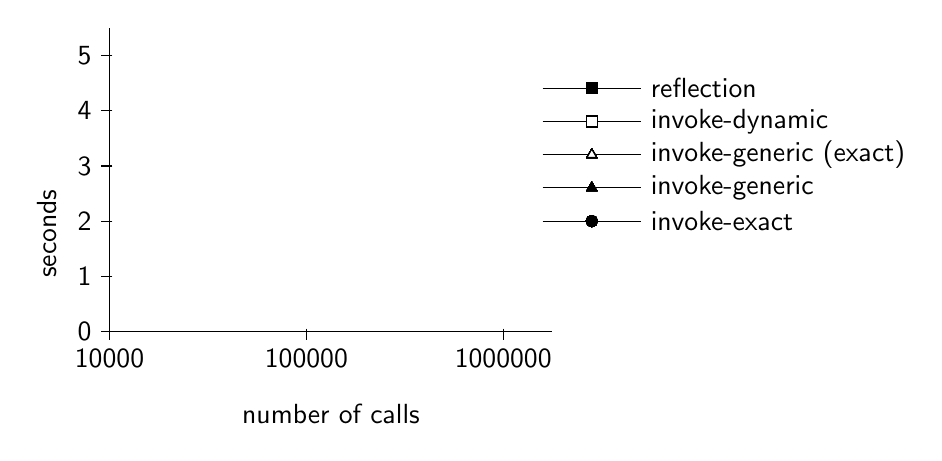
\begin{tikzpicture}[y=.7cm, x=2.5cm,font=\sffamily]
  %axis
  \draw (0,0) -- coordinate (x axis mid) (2.25,0);
      \draw (0,0) -- coordinate (y axis mid) (0,5.5);
      %ticks
      \draw (0,1pt) -- (0,-3pt) node[anchor=north] {10000};
      \draw (1,1pt) -- (1,-3pt) node[anchor=north] {100000};
      \draw (2,1pt) -- (2,-3pt) node[anchor=north] {1000000};
      \foreach \y in {0,...,5}
        \draw (1pt,\y) -- (-3pt,\y) node[anchor=east] {\y}; 
  %labels      
  \node[below=0.8cm] at (x axis mid) {number of calls};
  \node[rotate=90, left=.8cm] at (y axis mid) {seconds};

  %plots
  \draw plot[mark=*] 
    file {datas/exact.data};
  \draw plot[mark=triangle*] 
    file {datas/generic.data};
  \draw plot[mark=triangle*, mark options={fill=white}]
    file {datas/genexact.data};
  \draw plot[mark=square*, mark options={fill=white}]
    file {datas/dynamic.data};  
  \draw plot[mark=square*] 
    file {datas/reflection.data};  

  %legend
  \begin{scope}[shift={(2.2,2)}] 
    \draw (0,0) -- 
      plot[mark=*] (0.25,0) -- (0.5,0) node[right]{invoke-exact};
    \draw[yshift=\baselineskip] (0,0) -- 
      plot[mark=triangle*] (0.25,0) -- (0.5,0) node[right]{invoke-generic};
    \draw[yshift=2\baselineskip] (0,0) -- 
      plot[mark=triangle*, mark options={fill=white}] (0.25,0) -- (0.5,0) node[right]{invoke-generic (exact)};
    \draw[yshift=3\baselineskip] (0,0) -- 
      plot[mark=square*, mark options={fill=white}] (0.25,0) -- (0.5,0) node[right]{invoke-dynamic};
    \draw[yshift=4\baselineskip] (0,0) -- 
      plot[mark=square*] (0.25,0) -- (0.5,0) node[right]{reflection};
  \end{scope}
\end{tikzpicture}
}
    \caption{JSR 292 instructions vs reflection API}
    \label{Rinvoke}
  \end{figure}

  Figure \ref{Rinvoke} shows results for 10000, 100000 and 1000000.
  Below these values, we cannot see strictly differences between each kind of execution.
  We notice that calls to ``invoke-exact'' and to ``invoke-generic'' with the right method type (behaving as an ``invoke-exact'') are more faster than the others.
  ``invoke-dynamic'' takes a little more time because it have to get a volatile method handle.
  Regarding ``invoke-generic'' with a method type different to the final call, the execution time increase.
  This difference is due to conversions, more specifically, the boxing mecanism which creates new objects.
  However, ``invoke-generic'' remains more faster than the reflection API which requires to box all arguments and create an array of Object.\\
  
  An other test executes the example describes in this article.
  We call N times a method which takes an Object and calls the right method according to the dynamic type of the argument.
  We compare the execution time of the example using the instanceof mecanism, the reflection API and the method handle interpreter.

  \begin{figure}[!h]
    \resizebox{\linewidth}{!}{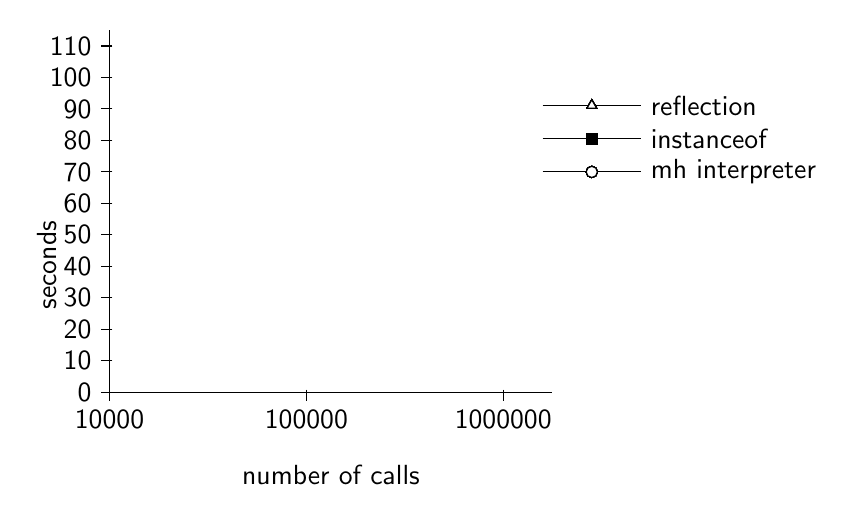
\begin{tikzpicture}[y=.04cm, x=2.5cm,font=\sffamily]
  %axis
  \draw (0,0) -- coordinate (x axis mid) (2.25,0);
      \draw (0,0) -- coordinate (y axis mid) (0,115);
      %ticks
      \draw (0,1pt) -- (0,-3pt) node[anchor=north] {10000};
      \draw (1,1pt) -- (1,-3pt) node[anchor=north] {100000};
      \draw (2,1pt) -- (2,-3pt) node[anchor=north] {1000000};
      \foreach \y in {0,10,...,110}
        \draw (1pt,\y) -- (-3pt,\y) node[anchor=east] {\y}; 
  %labels      
  \node[below=0.8cm] at (x axis mid) {number of calls};
  \node[rotate=90, left=0.8cm] at (y axis mid) {seconds};

  %plots
  \draw plot[mark=*, mark options={fill=white}] 
    file {mcs_indy.data};
  \draw plot[mark=square*]
    file {mcs_instanceof.data};
  \draw plot[mark=triangle*, mark options={fill=white}]
    file {mcs_reflection.data};  

  %legend
  \begin{scope}[shift={(2.2,70)}] 
    \draw (0,0) -- 
      plot[mark=*, mark options={fill=white}] (0.25,0) -- (0.5,0) node[right]{mh interpreter};
    \draw[yshift=\baselineskip] (0,0) -- 
      plot[mark=square*] (0.25,0) -- (0.5,0) node[right]{instanceof};
    \draw[yshift=2\baselineskip] (0,0) -- 
      plot[mark=triangle*, mark options={fill=white}] (0.25,0) -- (0.5,0) node[right]{reflection};
  \end{scope}
\end{tikzpicture}}
    \caption{Method handle interpreter vs instanceof vs reflection API}
    \label{Rmutable}
  \end{figure}

  We notice on the Figure \ref{Rmutable} our method handle interpreter is really slow.
  The method handle interpreter manipulates arguments.
  So it have to create an array each time it have to reduce or to increase the number of arguments.

\section{Related Works}

\appendix
\section{Appendix Title}

This is the text of the appendix, if you need one.

\section{Acknowledgments}

Acknowledgments, if needed.

% We recommend abbrvnat bibliography style.

\makeatletter
  \def\@seccntformat#1{Appendix~\csname the#1\endcsname:\quad}
\makeatother

% \bibliographystyle{abbrvnat}
\bibliographystyle{abbrv}

% The bibliography should be embedded for final submission.
\begin{thebibliography}{}
%   \softraggedright

  \bibitem{idc-website}
  IDC website (2013) - \\ \url{www.idc.com/getdoc.jsp?containerId=prUS24257413}

  \bibitem{lang-groovy}
  Groovy website - \\ \url{http://groovy.codehaus.org/}
  
  \bibitem{wiki-android}
  \ANDROID (Wikipedia) - \\ \url{en.wikipedia.org/wiki/Android\_(operating\_system)#Linux}

  \bibitem{wiki-jvm-lang}
  \JVM languages (Wikipedia) - \\ \url{https://en.wikipedia.org/wiki/List\_of\_JVM\_languages}
%   @ARTICLE{5676144, 
%   author={Butler, M.}, 
%   journal={Pervasive Computing, IEEE}, 
%   title={Android: Changing the Mobile Landscape}, 
%   year={2011}, 
%   volume={10}, 
%   number={1}, 
%   pages={4-7}, 
%   keywords={mobile computing;mobile radio;operating systems (computers);Android phones;Google;iPhone market;mobile landscape;smart phones;Androids;Driver circuits;Marketing and sales;Mobile communication;Smart phones;Android;App Inventor for Android;Apple App Store;BlackBerry;Technovation;iPhone}, 
%   doi={10.1109/MPRV.2011.1}, 
%   ISSN={1536-1268},}
  \bibitem{ieee-butler-android-landscape}
   Butler, M., ``Android: Changing the Mobile Landscape,'' Pervasive Computing, IEEE , vol.10, no.1, pp.4,7, Jan.-March 2011

%   @INPROCEEDINGS{5578292, 
%   author={Paul, K. and Kundu, T.K.}, 
%   booktitle={Computer and Information Technology (CIT), 2010 IEEE 10th International Conference on}, 
%   title={Android on Mobile Devices: An Energy Perspective}, 
%   year={2010}, 
%   pages={2421-2426}, 
%   keywords={Java;Linux;energy consumption;mobile handsets;operating system kernels;program compilers;public domain software;Android;Angstrom linux;\DALVIK JVM;Google;HTC;JAVA applications;Motorola;OHA;Sun;dynamic compiler;embedded devices;energy consumption;energy perspective;linux kernel;mobile devices;open handset alliance;open source platform;power management framework;Computers;Conferences;Information technology;Android Energy;\DALVIK JVM}, 
%   doi={10.1109/CIT.2010.416},}
  \bibitem{ieee-paul-kundu-energy-perspective}
  Paul, K.; Kundu, T.K., ``Android on Mobile Devices: An Energy Perspective,'' Computer and Information Technology (CIT), 2010 IEEE 10th International Conference on , vol., no., pp.2421,2426, June 29 2010-July 1 2010

  \bibitem{ieee-paulson-shift-dynamic-languages}
  Paulson, L.D., ``Developers shift to dynamic programming languages,'' Computer , vol.40, no.2, pp.12,15, Feb. 2007

%   \bibitem[Smith et~al.(2009)Smith, Jones]{smith02}
%   P. Q. Smith, and X. Y. Jones. ...reference text...

\end{thebibliography}


\end{document}

%                       Revision History
%                       -------- -------
%  Date         Person  Ver.    Change
%  ----         ------  ----    ------

%  2013.06.29   TU      0.1--4  comments on permission/copyright notices

